\documentclass{siamart190516}

% SIAM Shared Information Template
% This is information that is shared between the main document and any
% supplement. If no supplement is required, then this information can
% be included directly in the main document.


% Packages and macros go here
\usepackage{lipsum}
\usepackage{amsfonts}
\usepackage{amsmath}
\usepackage{amssymb}
\usepackage{graphicx}
\usepackage{epstopdf}
\usepackage{algorithmic}
\usepackage{enumerate}
\usepackage{dsfont}

\ifpdf
  \DeclareGraphicsExtensions{.eps,.pdf,.png,.jpg}
\else
  \DeclareGraphicsExtensions{.eps}
\fi

% Add a serial/Oxford comma by default.
\newcommand{\creflastconjunction}{, and~}
\newcommand{\prob}[1]{\mathds{P} \left( #1 \right)}
\newcommand{\inv}[1]{#1^{-1}}
\newcommand{\norm}[1]{\left| #1 \right|}
\newcommand{\ceil}[1]{\left\lceil #1 \right\rceil}

% Caligraphy Letters
\newcommand{\F}{\mathcal{F}}
\newcommand{\A}{\mathcal{A}}
\newcommand{\unif}{\mathcal{U}}

\DeclareMathOperator*{\argmax}{arg\,max}
\DeclareMathOperator*{\argmin}{arg\,min}

% Used for creating new theorem and remark environments
\newsiamremark{remark}{Remark}
\newsiamremark{hypothesis}{Hypothesis}
\crefname{hypothesis}{Hypothesis}{Hypotheses}
\newsiamthm{claim}{Claim}

% Sets running headers as well as PDF title and authors
\headers{6.437 Final Project | Part I}{Juan M Ortiz}

% Title. If the supplement option is on, then "Supplementary Material"
% is automatically inserted before the title.
\title{6.437 Final Project | Write up I}

% Authors: full names plus addresses.
\author{Juan M Ortiz}

\usepackage{amsopn}
\DeclareMathOperator{\diag}{diag}

\graphicspath{{figures}}

% Optional PDF information
\ifpdf
\hypersetup{
  pdftitle={6.437 Final Project Part I},
  pdfauthor={Juan M Ortiz}
}
\fi

\begin{document}
\maketitle

\section*{Problem I: A Bayesian Framework}
\label{sec:bayesian}


\begin{enumerate}[(a)]

  % Part A
  \item \begin{align*}
          p_{\textbf{y}|f}(\textbf{y}|f) & = \prob{ \textbf{x}_0 = \inv{f}(\textbf{y}_0)} \prod_{j = 1}^{n-1} \prob{\textbf{x}_j = \inv{f}(y_j) | \textbf{x}_{j-1} = \inv{f}} \\
                                         & = p_{\inv{f}(y)}(\inv{f}(\textbf{y}_0)) \prod_{j = 1}^{n-1} M_{\inv{f}(\textbf{y})_{j}, \inv{f}(\textbf{y})_{j-1}}
        \end{align*}

        % Part B
  \item \begin{align*}
          p_{f|\textbf{y}}(f | \textbf{y}) & = \frac{ p_{\textbf{y}|f}(\textbf{y}|f) p_{f}(f) }{p_\textbf{y}(y)}                                                                                                                                                                                  \\
                                           & = \frac{p_{\inv{f}(y)}(\inv{f}(\textbf{y}_0)) \prod_{j = 1}^n M_{\inv{f}(\textbf{y})_{j}, \inv{f}(\textbf{y})_{j-1}}}{\sum_{g \in \F}(p_{\inv{g}(y)}(\inv{g}(\textbf{y}_0)) \prod_{j = 1}^n M_{\inv{g}(\textbf{y})_{j}, \inv{g}(\textbf{y})_{j-1}})}
        \end{align*}
        Where $\F$ is the set of all permutations of $\mathcal{A}$. Thus, the MAP estimator is one that maximizes the above expression or, equivalently, its numerator. Thus
        \[
          \hat{f}_{MAP} = \argmax_{f \in \F} p_{\inv{f}(y)}(\inv{f}(\textbf{y}_0)) \prod_{j = 1}^n M_{\inv{f}(\textbf{y})_{j}, \inv{f}(\textbf{y})_{j-1}}
        \]

        % Part C
  \item Direct computation of the $\hat{f}_{MAP}$ is infeasable because it requires an optimization over a large, discrete, non-linear set. Computing expression on (b) would optimize over $\F$ which has a size of $\norm{\F} = \norm{\mathcal{A}}! = 28! \simeq 10^{29}$. Additionally, the constraints necessary to enforce that the $f \in \F$ is permutation will be hard to optimize over.
\end{enumerate}

\section*{Problem 2: Markov Chain Monte Carlo method}
\label{sec:mcmc}
\begin{enumerate}[(a)]
  % Part A
  \item After the first fixing one of the two cyphering functions $f_1 \in \F$, there are $\binom{\norm{\mathcal{A}}}{2}$ possible $f_2 \in \F$ such that g differs in exactly two symbol assignments (i.e. those that swap two distinct element assignments in $f_1$). Thus, the probability that $f_1$ and $f_2$ differ in exactly two symbol assignments is given by:

        \[
          \frac{\binom{\mathcal{A}}{2}}{\norm{A}!} = \frac{1}{2(\norm{A} - 2)!}
        \]

        % Part B
  \item First, notice that the distribution $p_{f | \textbf{y}}$ can be factorized in to hold the form $p_{f | \textbf{y}}(f | \textbf{y}) = \frac{1}{Z}\tilde{p}_{f | \textbf{y}}$ where
        \begin{align*}
          \tilde{p}_{f | \textbf{y}} & = p_{\inv{f}(y)}(\inv{f}(\textbf{y}_0)) \prod_{j = 1}^n M_{\inv{f}(\textbf{y})_{j}, \inv{f}(\textbf{y})_{j-1}}                  \\
          Z                          & = \sum_{g \in \F}(p_{\inv{g}(y)}(\inv{g}(\textbf{y}_0)) \prod_{j = 1}^n M_{\inv{g}(\textbf{y})_{j}, \inv{g}(\textbf{y})_{j-1}})
        \end{align*}

        If we let the proposal distribution $V(f' | f)$ be defined as
        \[
          V(f' | f) = \begin{cases}
            \binom{\norm{\A}}{2}^{-1} \text{  for f and f' differ in exactly two symbol assignments} \\
            0 \text{  otherwise}
          \end{cases}
        \]

        When executing Metropolis-Hastings we compute the acceptance factor as follows:

        \begin{align*}
          a(f \rightarrow f') & \triangleq \min(1, \frac{\tilde{p}_{f | \textbf{y}}(f' | \textbf{y})}{\tilde{p}_{f | \textbf{y}}(f | \textbf{y})} \frac{V(f | f')}{V(f' | f)}) \\
                              & =\min(1, \frac{\tilde{p}_{f | \textbf{y}}(f' | \textbf{y})}{\tilde{p}_{f | \textbf{y}}(f | \textbf{y})})
        \end{align*}

        Note that in the event that $\tilde{p}_{f | \textbf{y}}(f' | \textbf{y}) = \tilde{p}_{f | \textbf{y}}(f' | \textbf{y}) = 0$, we will define $a(f \rightarrow f') = 1$.

        % Part C
  \item
        \begin{algorithm*}
          \caption{Decoding using Metropolis-Hastings}
          \label{alg:decoding}
          \begin{algorithmic}
            \STATE $\hat{\F} \leftarrow \{\}$
            \STATE $f \leftarrow$ random permutation of $\A$

            \WHILE{$\norm{\hat{\F}} < 5000$}
            \STATE $f' \leftarrow$ permutation obtained by swapping two assignments of $f$ at random.
            \STATE $a(f \rightarrow f') \leftarrow \min(1, \frac{\tilde{p}_{f | \textbf{y}}(f' | \textbf{y})}{\tilde{p}_{f | \textbf{y}}(f | \textbf{y})})$
            \STATE $r \sim \unif(0, 1)$
            \IF{$r \leq a(f \rightarrow f')$}
            \STATE $\hat{\F} = \hat{\F} \cup \{ f' \}$
            \STATE $f \leftarrow f'$
            \ENDIF
            \ENDWHILE

            \STATE $f_{MAP} = \argmax_{f \in \hat{\F}} \tilde{{p}}_{f | \textbf{y}}(f | \textbf{y})$
            \RETURN $\inv{f_{MAP}}(\textbf{y})$
          \end{algorithmic}
        \end{algorithm*}
\end{enumerate}

\section*{Problem 3: Implementation}
\label{sec:experiments}

\begin{enumerate}[(a)]
  \item Log-likelihood v. Iteration Count\\
        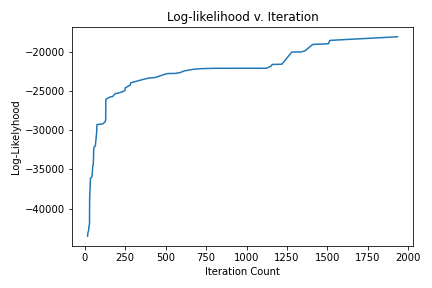
\includegraphics[width=5cm]{loglikelihoodviter.png}

        Note that in order to make convergence slightly faster, algorithm \ref{alg:decoding} was modified slightly by initializing the first permutation function to the permutation that matches the permutation that ensures that the ordering produced by the letter frequencies in P matches that of the emperical frequencies in the decoded ciphertext.

  \item Acceptance Rate (T = 100) v. Iteration Count \\
        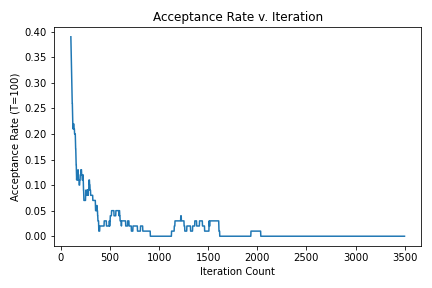
\includegraphics[width=5cm]{acceptancerateviter.png}
  \item Accuracy Rate v. Iteration Count\\
        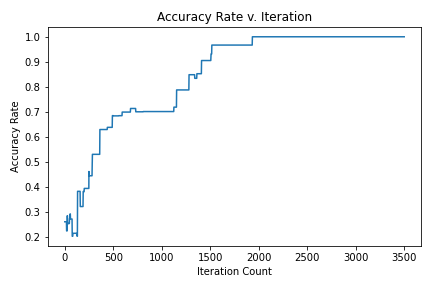
\includegraphics[width=5cm]{accuracyrateviter.png}
  \item The plot below depicts the average accuracy of decoded text as a function of the percent of the symbols of the ciphertext used. For each decoding run, the first $N * f$ symbols were used where $f$ is the fraction of sybmols to be utilized during the run. For each fraction to tested, the average accuracy was computed over $\ceil{\frac{1}{f}}$ runs.

        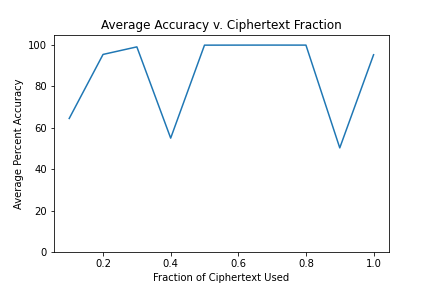
\includegraphics[width=5cm]{accvfrac.png}

        In general, the accuracy of the decoded text is highest when the entire ciphertext is used. This is because the longer the text, the fewer the permutations that generate an encoding that closely matches the true ciphertext. Thus, we have a higher probability of sampling an accurate ciphering function.

        Note that the above graph does not always follow this conclusion however. This is partly due to randomness and the fact that, for a shorter text, one can achieve a high accuracy even if the ciphering function is not accurate for a small portion of the encoded text.

  \item As the number of incresases, the log-likelihood per symbol seems to approach a number close to $-3.4$. This suggests that emperical entropy per symbol is approximatelly 3.4 bits per symbol. Note this is higher than the reported entropy of english in the reference article of approximatelly one bit per symbol mostly due to our modeling choice of only taking into account the immediatelly preceding symbol.

        The below plot depicts the evolution of the log-likelihood per symbol as we continue to iterate using (a slightly optimized version of) algorithm \ref{alg:decoding}.

        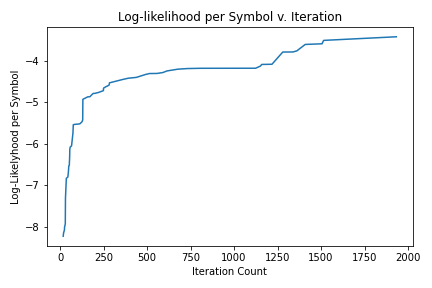
\includegraphics[width=5cm]{loglikelihoodviterpersymb.png}

\end{enumerate}

\end{document}
